\chapter{{Edge AI System Design \& Implementation}}

\section{System Overview and Methodology}

This chapter presents the design, implementation, and deployment of an edge AI-based grape leaf disease detection system into existing vineyard monitoring infrastructure. The proposed system extends conventional LoRaWAN-based wireless sensor networks, which monitors only environmental parameters, by integrating sensor-level deep learning inference to enable real-time plant health status assessment.



\subsection{Four-Stage Pipeline Architecture}

The disease detection system is implemented in a four-stage pipeline deployed on ESP32-S3 microcontrollers, as illustrated in Figure~\ref{fig:system_architecture}.

\begin{figure}[htbp]
    \centering
    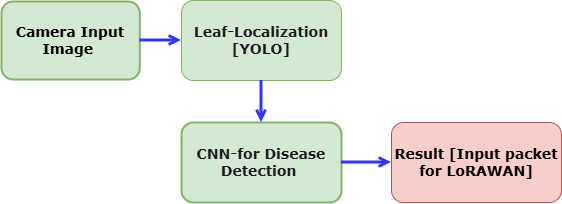
\includegraphics[width=0.75\linewidth]{images/system_architecture.png}

    \caption{Four-stage edge AI pipeline for grape leaf disease detection.}
    \label{fig:system_architecture}
\end{figure}

\textbf{Stage 1: Image Acquisition} -- An OV3660 camera module captures vineyard images at VGA resolution. The camera's built-in hardware JPEG encoder compresses images on-chip before transfer to the ESP32-S3.

\textbf{Stage 2: Leaf Localization} -- A YOLO-based detection model (ESPDet-Pico) localizes individual grape leaves within the captured frame. This stage identifies and crops leaf regions of interest, filtering out background elements. The ESP-optimized model architecture and training procedure are detailed in Section~\ref{sec:espdet_pico}.

\textbf{Stage 3: Disease Classification} -- Each detected leaf is resized and classified by a MobileNetV2 model fine-tuned on grape disease images. The two-stage transfer learning strategy and model evaluation are presented in Section~\ref{sec:mobilenetv2}.

\textbf{Stage 4: Multi-Leaf Aggregation} -- Since frames contain multiple leaves, predictions are aggregated using weighted combination of detection confidence, classification entropy, and spatial quality metrics. The aggregated result is encoded into a 16-byte LoRaWAN packet. The aggregation strategy and its effectiveness are analyzed in Chapter~\ref{chap:results}.



\section{Dataset Acquisition and Preparation}
\label{sec:dataset}
\vspace{-1mm}
In training the two distinct models, two separate datasets were used. The dataset for disease classification contains only single leaf images in a clear background, while the dataset for leaf localization contains images of natural vineyard scenes with annotated leaf bounding boxes. The reason for having two separate datasets is that the disease classification model is trained on a controlled dataset to learn disease-specific features on single leaf without background noise. But in practice the input image is natural vineyard scene with multiple leaves and complex background, so the leaf localization model is trained on a different dataset that reflects the deployment conditions to learn to localize leaves in unconstrained environments. Then the disease classification model is applied only on the detected \& cropped leaf regions obtained from the localization model, which is why it is trained on single leaf images. This separation allows each model to specialize in its respective task while ensuring that the overall system can handle real-world vineyard imagery effectively.
\vspace{-2mm}
\subsection{The Grape-Leaf Disease Dataset}
\vspace{-2mm}
The grape-leaf disease dataset obtained from the PlantVillage Dataset hosted on Kaggle~\cite{plantvillage_dataset_2023}, created by Abdallah Ali. PlantVillage is a widely-adopted public repository of plant disease imagery developed through collaborative citizen science efforts. The grape leaf subset aggregates pathology images captured under controlled laboratory conditions, ensuring consistent lighting and background characteristics. The dataset emphasizes leaf-level disease manifestations across four epidemiologically significant categories affecting viticulture worldwide. The dataset contains 4,062 RGB images and is distributed across four distinct disease classes: \textit{Black Rot} (caused by \textit{Guignardia bidwellii}), \textit{Esca} (Black Measles, a complex disease involving multiple fungal pathogens), \textit{Leaf Blight} (Isariopsis Leaf Spot, caused by \textit{Pseudocercospora vitis}), and  finally the \textit{Healthy class} (disease-free sample of grape leaves). Table~\ref{tab:classification_dataset_distribution} presents the complete class distribution statistics. 

\begin{table}[htbp]
\centering
\caption{Grape leaf disease dataset distribution across training, validation, test splits}
\label{tab:classification_dataset_distribution}
\begin{tabular}{lrrrr}
\toprule
\textbf{Disease Class} & \textbf{Training} & \textbf{Validation} & \textbf{Test} & \textbf{Total} \\
\midrule
Black Rot              & 803               & 141                 & 236           & 1,180          \\
Esca (Black Measles)   & 940               & 166                 & 277           & 1,383          \\
Healthy                & 287               & 51                  & 85            & 423            \\
Leaf Blight            & 731               & 129                 & 216           & 1,076          \\
\midrule
\textbf{Total}         & \textbf{2,761}    & \textbf{487}        & \textbf{814}  & \textbf{4,062} \\
\bottomrule
\end{tabular}
\end{table}

The dataset employs a fixed 80/20 train-test split at the top level, allocating 3,248 images for model development and 814 images for final evaluation. Stratified sampling ensures proportional class representation in both partitions, maintaining the original class distribution ratios. The development partition (3,248 images) is further subdivided into 85\% for training (2,761 images) and 15\% for validation (487 images), as detailed in Table~\ref{tab:classification_dataset_distribution}. This three-way split enables hyperparameter tuning on the validation set while preserving the test set for unbiased performance evaluation. All splits maintain class balance through stratified partitioning to prevent training bias toward majority classes.

\subsection{Grapevine Dataset for Leaf Localization}

The leaf localization dataset is used to train a model to identify grape leaf regions of interest (ROI) within unconstrained vineyard imagery. Unlike the classification dataset's controlled backgrounds, this dataset includes natural vineyard scenes with complex backgrounds, occlusions, and varying lighting conditions. These base images are sourced from the Grape/Grapes dataset on Kaggle~\cite{kaggle_grape_images_2023}, curated by Nicolaas Regnier. This collection contains 531 natural vineyard photographs capturing real-world deployment conditions with varying leaf densities, overlaps, lighting conditions, and background complexity. Unlike the disease classification dataset, which contains single leaves on uniform backgrounds, this collection captures the unstructured complexity of real vineyard environments, essential for training robust leaf localization models.

To adapt this dataset for object detection training, the images were manually annotated with bounding boxes of individual grape leaf regions. The annotation process was conducted using the Roboflow platform and segment anything model (SAM), where each leaf instance within the images was labeled with precise bounding box coordinates. These annotations are based on the YOLO format, each bounding boxes are specified by normalized center coordinates $(x_c, y_c)$, width $w$, and height $h$, all scaled to $[0, 1]$ relative to image dimensions. This normalization ensures resolution-independent annotation representation, facilitating training across variable input sizes. The annotated dataset, titled ``Grape Leaf ROI Detection'' is publicly published on Roboflow platform~\cite{roboflow_grape_leaf_2026}. The dataset exported in YOLOv11 format compatible with modern object detection frameworks. This dataset partitioned into training (328 images), validation (82 images), and test (103 images) sets, maintaining the natural distribution of leaf counts and scene complexity across splits. 


\subsection{Preprocessing and Augmentation Pipeline}

Data preprocessing and augmentation strategies differ substantially between the classification and detection tasks due to their distinct architectural requirements, input constraints, and training objectives.

\subsubsection{Input Resolution and Preprocessing}

Hardware memory limitations of the ESP32-S3 platform impose strict constraints on input resolution selection. The classification model operates on $128 \times 128$ pixel inputs, balancing model expressiveness with PSRAM availability for activation storage during inference. The detection model processes rectangular inputs at $416 \times 320$ pixels (aspect ratio 1.3:1), selected to accommodate the OV3660 camera's VGA output while maintaining computational efficiency for multi-object detection.

For classification, training images undergo \texttt{RandomResizedCrop} to $128 \times 128$ pixels, enabling scale augmentation. Validation and test images are deterministically resized to $144 \times 144$ pixels, then center-cropped to $128 \times 128$ to extract the most salient region. For detection, images are resized to $416 \times 320$ using aspect-ratio-preserving letterboxing~\cite{redmon2016yolo}: shorter dimension is scaled to target size, and the longer dimension is padded with gray pixels ($[114, 114, 114]$) to achieve rectangular dimensions without distortion. This rectangular training strategy~\cite{bochkovskiy2020yolov4} reduces computational cost compared to square inputs while maintaining aspect ratio fidelity.

\subsubsection{Normalization and Standardization}

All images undergo channel-wise normalization using ImageNet dataset statistics~\cite{deng2009imagenet}: mean $\mu = [0.485, 0.456, 0.406]$ and standard deviation $\sigma = [0.229, 0.224, 0.225]$ for RGB channels. This normalization practice, established by Krizhevsky et al.~\cite{krizhevsky2012imagenet}, aligns input distributions with the pre-training regime of transfer learning base models (MobileNetV2~\cite{sandler2018mobilenetv2} for classification, YOLO11n~\cite{ultralytics2024yolo11} for detection), accelerating convergence during domain adaptation. The normalization transformation is defined as:
\begin{equation}
x_{\text{norm}} = \frac{x / 255 - \mu}{\sigma}
\end{equation}
where $x \in [0, 255]$ represents raw pixel intensities. This standardization centers the distribution around zero and scales variance to unity, stabilizing gradient flow during backpropagation~\cite{ioffe2015batchnorm}.

\subsubsection{Online Data Augmentation Strategy}

Data augmentation is applied \textit{online} (on-the-fly) during training rather than offline preprocessing. Online augmentation generates stochastically transformed samples at each epoch, enabling infinite dataset variation from a finite set of images without storage overhead~\cite{shorten2019survey}. This approach is critical for moderate-sized datasets where offline augmentation would require prohibitive disk space (e.g., $10 \times$ augmentation of 4,062 images yields 40,620 stored variants). Furthermore, online augmentation introduces randomness across epochs, preventing the model from memorizing specific augmented variants and improving generalization~\cite{perez2017effectiveness}.

Implementation uses PyTorch's \texttt{torchvision.transforms} module~\cite{pytorch2019} for classification and Ultralytics' built-in augmentation pipeline~\cite{ultralytics2024yolo11} for detection, both applying transformations during data loading via \texttt{DataLoader} workers in parallel to GPU training.

\subsubsection{Task-Specific Augmentation: Disease Classification}

Classification training employs aggressive augmentation to mitigate overfitting on the 4,062-image dataset and enhance robustness to field deployment variability. The augmentation pipeline comprises nine transformations applied sequentially with stochastic activation:

\begin{enumerate}
    \item \textbf{RandomResizedCrop}$(128 \times 128, \text{scale}=[0.5, 1.0])$: Extracts random crops spanning 50\%--100\% of original area, then resizes to $128 \times 128$. Simulates varying camera-to-leaf distances and leaf size diversity.
    
    \item \textbf{RandomHorizontalFlip}$(p=0.5)$: Horizontal mirroring with 50\% probability, exploiting bilateral symmetry of vineyard row arrangements.
    
    \item \textbf{RandomVerticalFlip}$(p=0.2)$: Vertical mirroring with 20\% probability, accommodating arbitrary camera mounting orientations.
    
    \item \textbf{RandomRotation}$(\pm 25^\circ)$: Uniform rotation within $[-25^\circ, +25^\circ]$, addressing non-upright leaf poses and camera roll variations.
    
    \item \textbf{ColorJitter}$(b=0.5, c=0.5, s=0.5, h=0.15)$: Randomly perturbs brightness, contrast, saturation (each $\pm 50\%$), and hue ($\pm 15\%$). Critical for robustness to diurnal illumination changes, cloud shadows, and sensor white-balance variations in outdoor deployments~\cite{buslaev2020albumentations}.
    
    \item \textbf{RandomPerspective}$(\text{distortion}=0.3, p=0.4)$: Applies perspective warping with 40\% probability and distortion scale 0.3, simulating oblique viewing angles when leaves are not perpendicular to camera optical axis.
    
    \item \textbf{RandomGrayscale}$(p=0.15)$: Converts to grayscale with 15\% probability, forcing model to learn texture and shape cues independent of color, improving robustness to color-insensitive disease symptoms.
    
    \item \textbf{GaussianBlur}$(\text{kernel}=3, \sigma \in [0.1, 1.5])$: Applies Gaussian blur with random $\sigma$ to simulate slight defocus or motion blur from wind-induced leaf movement.
    
    \item \textbf{RandomErasing}$(p=0.3, \text{area}=[0.02, 0.15])$: Randomly erases 2\%--15\% of image area with 30\% probability, encouraging robustness to partial occlusions (e.g., overlapping leaves, insects, dust)~\cite{zhong2020randomerasing}.
\end{enumerate}

All transformations are applied probabilistically during each training iteration via PyTorch's \texttt{transforms.Compose}, with independent random seeds per sample to maximize diversity.

\subsubsection{Task-Specific Augmentation: Leaf Localization}

Detection training employs YOLO-specific augmentations optimized for multi-scale object localization. The augmentation strategy balances robustness with localization precision, as excessive distortion degrades bounding box regression accuracy. The pipeline includes:

\begin{itemize}
    \item \textbf{Geometric Augmentations}: Rotation ($\pm 10^\circ$), translation ($\pm 10\%$), scale ($0.5 \times$--$1.5 \times$), shear ($\pm 2^\circ$), horizontal/vertical flips ($p=0.5$ each). Conservative ranges prevent extreme distortions that misalign bounding boxes.
    
    \item \textbf{Photometric Augmentations}: HSV jitter with minimal hue shift ($\pm 1.5\%$), moderate saturation/value adjustments ($\pm 40\%$). Reduced intensity compared to classification, as detection focuses on structural features rather than disease-specific color.
    
    \item \textbf{Mosaic Augmentation}~\cite{bochkovskiy2020yolov4}: Combines four images into a single training sample with 50\% probability, enhancing multi-scale learning and small-object detection. Disabled after epoch 50 (close\_mosaic=50) to fine-tune on full-resolution images.
    
    \item \textbf{MixUp}$(p=0.05)$: Blends two images linearly with 5\% probability, regularizing the model through label smoothing~\cite{zhang2018mixup}. Low probability prevents over-smoothing that harms localization.
    
    \item \textbf{Copy-Paste}$(p=0.15)$: Randomly pastes leaf instances from other images with 15\% probability, augmenting object count and contextual diversity~\cite{ghiasi2021copypaste}.
\end{itemize}

Augmentations are implemented via Ultralytics' internal pipeline, applied during data loading with rectified batch sampling to maintain $416 \times 320$ aspect ratio across batches~\cite{ultralytics2024yolo11}.

\subsubsection{Validation and Test Preprocessing}

Validation and test sets receive only deterministic preprocessing without stochastic augmentation. For classification: resize to $144 \times 144$, center-crop to $128 \times 128$, normalize. For detection: letterbox resize to $416 \times 320$, normalize. This augmentation-free protocol ensures performance metrics reflect true model generalization on canonical inputs, avoiding artificially inflated accuracies from test-time augmentation~\cite{krizhevsky2012imagenet}. The separation of augmented training data from clean evaluation data maintains rigorous evaluation standards consistent with machine learning best practices.



\section{Hardware Platform Selection}
\label{sec:hardware}

\subsection{ESP32-S3 System Architecture}
% Processor architecture and computational capabilities
% Memory subsystem organization (SRAM, PSRAM)
% Integrated peripherals relevant to deployment

\subsection{Hardware Selection Rationale}
% Edge AI platform comparison (embedded MCU vs SBC)
% Cost, power, and memory trade-off analysis
% Agricultural deployment constraints



\section{Leaf Localization Model Design}
\label{sec:espdet_pico}

\subsection{Object Detection Framework Selection}
% YOLO architecture family overview
% YOLO11n baseline characteristics
% Baseline performance and resource requirements

\subsection{Model Compression for Embedded Deployment}
% ESPDet-Pico architectural modifications
% Pruning and layer reduction strategies
% Quantization-aware training

\subsection{Training Methodology}
% Training dataset characteristics and split
% Hyperparameter configuration
% Loss function and optimization strategy
% Convergence behavior and early stopping

\subsection{Detection Performance Evaluation}
% Mean Average Precision (mAP@50) analysis
% Precision-recall characteristics
% ESPDet-Pico vs YOLO11n comparative analysis
% Accuracy-memory trade-off justification



\section{Disease Classification Model Design}
\label{sec:mobilenetv2}

\subsection{Convolutional Neural Network Architecture}
% MobileNetV2 depthwise separable convolution design
% Inverted residual blocks and linear bottlenecks
% Architectural efficiency vs ResNet-18 comparison
% Pre-trained weight initialization (ImageNet)

\subsection{Transfer Learning Strategy}
% Domain adaptation from natural images to plant pathology
% Two-stage progressive fine-tuning (Stage 1 & Stage 2)
% Learning rate scheduling and decay strategy

\subsection{Training Protocol}
% Optimizer configuration (AdamW)
% Loss function and regularization
% Training duration and convergence criteria
% Multi-seed experimental protocol

\subsection{Classification Accuracy and Robustness}
% Test set performance across multiple training runs
% Statistical analysis of model stability
% Per-class performance metrics (precision, recall, F1-score)
% Confusion matrix interpretation

\subsection{Post-Training Quantization}
% ESP-PPQ quantization framework
% FP32 to INT8 conversion methodology
% Quantization accuracy degradation analysis
% Final model size and memory footprint



\section{System Integration and Embedded Deployment}
\label{sec:deployment}

\subsection{Memory Management Architecture}
% SRAM allocation strategy for time-critical operations
% PSRAM allocation for model weights and activations
% Dynamic buffer management for multi-stage pipeline
% Memory fragmentation mitigation

\subsection{Inference Pipeline Implementation}
% Multi-stage inference orchestration
% Inter-stage data dependencies and synchronization
% Preprocessing, detection, classification, and aggregation workflow
% Resource sharing and buffer reuse

\subsection{Computational Performance Characterization}
% Per-stage latency profiling
% Inference throughput analysis
% Computational bottleneck identification
% Multi-leaf inference scaling behavior










